Poslednje pravilo, ki ga je potrebno vpeljati, je \emph{pravilo reza}. To pravilo obstaja tudi v običajnem sekventnem računu in formalizira koncept dokazovanja s pomočjo leme.

\begin{definicija}
	\emph{Pravilo reza}, krajše $Rez$:
	\begin{prooftree}
        \AxiomC{$\Gamma \Rightarrow A,\Delta$}
        \AxiomC{$\Gamma',A \Rightarrow \Delta'$}
        \pravilo{Rez}
        \BinaryInfC{$\Gamma,\Gamma' \Rightarrow \Delta,\Delta'$}
	\end{prooftree}
	To pravilo pravi, da če znamo pod določenimi predpostavkami dokazati formulo $A$, potem pa iz te formule dokažemo nekaj drugega, lahko $A$ enostavno režemo iz procesa.
\end{definicija}

\begin{opomba}
    Sekventni račun brez uporabe pravila reza ima pomembno lastnost, namreč da vsak dokaz sekventa $\Gamma \Rightarrow \Delta$ v svoji izpeljavi uporabi le podformule formul, ki nastopajo v $\Gamma$ in $\Delta$. To je osnova za mnoge algoritme, ki iščejo dokaze, pa tudi sicer ima ta lastnost mnogo koristnih posledic.??lahko dam to tukaj??. Ko vpeljemo pravilo reza, se ta lastnost izgubi, saj lahko na vsakem koraku ,,vrinemo'' poljubno formulo.
\end{opomba}

Če pravilo reza res interpretiramo kot uporabo leme, bi imelo smisel sklepati, da z uporabo rezov ne moremo pridelati sekventov, ki jih brez tega pravila nismo mogli dokazati. Ravno temu služi naslednji izrek.

\begin{izrek}[Izrek o eliminaciji rezov] \label{izrek}
    Vsak sekvent, izpeljan z uporabo reza, lahko izpeljemo tudi brez uporabe reza.
\end{izrek}

\subsection{Potrebne definicije} \label{defs}
Dokaz zgornjega izreka poteka s pomočjo indukcije na drevesih izpeljave nad rezom ter na kompleksnosti formul, ki jih režemo. Zavoljo tega moramo tako na drevesih kot formulah vpeljati nekakšno mero, glede na katero bomo potem izvalali proces indukcije. Formula je induktivno definirana v definiciji \ref{formula}, zato je tudi kompleksnost formule definirana induktivno.

\begin{definicija}
    Naj bosta $A$ in $B$ poljubni formuli, $P$ pa naj bo neka osnovna formula. \emph{Rang formule}, označen s simbolom $\R$, je definiran sledeče:
    \begin{itemize}
        \item $\R(P) = \R(\top) = \R(\bot) = \R(\enota) = \R(\nicla) = 1$
        \item $\R(\negacija A) = \R(\forall x A) = \R(\exists x A) = \R(A) + 1$
        \item $\R(A*B) = \max\{\R(A),\R(B)\} + 1$ ; kjer je $*$ poljuben veznik, ki sprejme dve formuli.
    \end{itemize}
\end{definicija}

Podobno je definirana višina drevesa. Imejmo naslednji dve drevesi, levo označeno z $\D$, desno pa z $\D'$:
\begin{center}
    \begin{bprooftree}
        \AxiomC{$\D_0$}
        \AxiomC{$\D_1$}
        \AxiomC{$\ldots$}
        \AxiomC{$\D_n$}
        \pravilo{Pravilo}
        \QuaternaryInfC{$\mathcal{S}$}
    \end{bprooftree}
    \begin{bprooftree}
        \AxiomC{}
        \pravilo{Pravilo'}
        \UnaryInfC{$\mathcal{S}$'}
    \end{bprooftree}
\end{center}
Tu je $n\in\mathbb{N}$, Pravilo je poljubno pravilo, ki sprejme $n$ sekventov, Pravilo' pa je poljubno pravilo, ki jih ne sprejme nič. Slednje je na primer pravilo aksioma ali nekatera izmed pravil za konstante:

\begin{definicija}
    \emph{Višina drevesa izpeljave} je označena s simbolom $\h$ in je enaka:
    \begin{itemize}
        \item$\h(\D) = \max\{\h(\D_0),\h(\D_1),\ldots,\h(\D_n)\} + 1$
        \item$\h(\D') = 1$
    \end{itemize}
\end{definicija}

Sedaj ko imamo mero tako na formulah kot na drevesih izpeljave, lahko defniramo skupno mero vsakega reza. Oglejmo si poljubno pravilo reza:
\begin{prooftree} \label{rez general}
    \AxiomC{$\D_0$}
    \noLine
    \UnaryInfC{$\Gamma,A \Rightarrow \Delta$}

    \AxiomC{$\D_1$}
    \noLine
    \UnaryInfC{$\Gamma' \Rightarrow A,\Delta'$}

    \pravilo{Rez}
    \BinaryInfC{$\Gamma,\Gamma' \Rightarrow \Delta,\Delta'$}
\end{prooftree}
Tu $\D_0$ in $\D_1$ označujeta drevesi izpeljav, ki sta vodili do sekventov pod njima.

\begin{definicija} \label{stopnja}
    \emph{Stopnja reza} je par števil $(\R,\h)$, kjer je $\R$ rang rezane formule, $\h$ pa višina samega drevesa. Z zgornjimi oznakami je stopnja reza torej enaka:
    $$
    (\R,\h) = (\R(A), \max\{\h(\D_0),\h(\D_1)\} + 2)
    $$
    Stopnja reza je urejena \emph{leksikografsko}, kar pomeni, da relacijo < na paru $(\R,\h)$ definiramo sledeče:
    $$
    (\R,\h) < (\R',\h') \Leftrightarrow (\R < \R') \text{ ali } ((\R = \R') \text{ in } (\h < \h'))
    $$
\end{definicija}
\begin{definicija} \label{najnizji}
    Rezu bomo rekli \emph{najnižji rez}, če se nad njim ne pojavi nobeno drugo pravilo reza. To seveda ne pomeni nujno, da ima najnižjo stopnjo ali da je v drevesu izpeljave le en takšen rez.
\end{definicija}

Preden začnemo z dokazom je nazadnje potrebno definirati še eno vrsto reza, in sicer glavni rez.

\begin{definicija} \label{gl rez}
    Če je rezana formula vpeljana v obeh poddrevesih nad pravilom reza, to imenujemo \emph{glavni rez}.
\end{definicija}

\begin{primer*} \label{gl rez in}
    Glavni rez za formulo $A \sqcap B$.
    \begin{prooftree}
        \AxiomC{$\Gamma,A \Rightarrow \Delta$}
        \levopravilo{L$\sqcap$}
        \UnaryInfC{$\Gamma,A \sqcap B \Rightarrow \Delta$}

        \AxiomC{$\Gamma' \Rightarrow A,\Delta'$}
        \AxiomC{$\Gamma' \Rightarrow B,\Delta'$}
        \pravilo{R$\sqcap$}
        \BinaryInfC{$\Gamma' \Rightarrow A \sqcap B,\Delta'$}

        \pravilo{Rez}
        \BinaryInfC{$\Gamma,\Gamma' \Rightarrow \Delta,\Delta'$}
    \end{prooftree}
\end{primer*}


\subsection{Dokaz izreka o eliminaciji rezov} \label{dokaz}

Izrek 4.3 imenujemo izrek o \emph{eliminaciji} rezov, ker v njegovem dokazu postopoma odstranjujemo (eliminiramo) reze iz drevesa izpeljave, dokler nam na koncu ne ostane drevo izpeljave brez rezov. Dokaz poteka z dvojno indukcijo, zunanjo na številu rezov v dokazu, notranjo pa na stopnji reza, kot je definirana v \ref{stopnja}.

Začnimo z indukcijo na številu rezov. Če je drevo brez rezov, smo dokaz končali. Bazi indukcije, torej primeru ko je $n=0$, smo tako avtomatično zadostili. Sedaj denimo, da imamo v drevesu izpeljave $n+1$ rezov. Ker je to drevo končno, si lahko izberemo enega izmed najnižjih rezov, denimo mu Rez$_0$. Oglejmo si poddrevo, ki se konča z Rez$_0$:
\begin{figure}[h]
    \centering 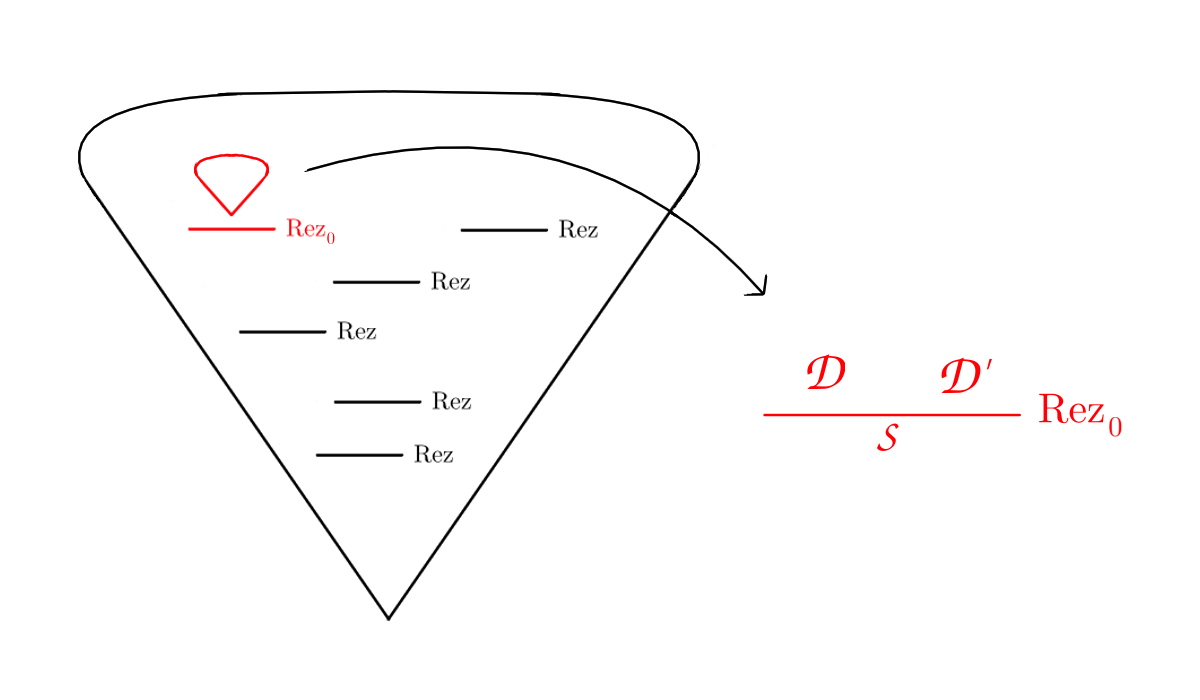
\includegraphics{polj_drevo.png}
\end{figure}

Drevesi $\D$ in $\D'$ ne vsebujeta pravila rez. Če znamo torej eliminirati rez iz takšnega poddrevesa, lahko zgornje drevo izpeljave prevedemo na drevo, ki vsebuje le $n$ rezov. Po indukcijski predpostavki znamo sedaj eliminirati še ostale reze. Dokaz eliminacije rezov smo tako prevedli na dokaz eliminacije rezov iz drevesa, kjer je zadnje pravilo rez, nad njim pa ni drugih rezov.

Za eliminiacijo zgoraj opisanega reza pa potrebujemo indukcijo na stopnjo reza. Indukcijski ķorak poteka tako, da drevo, ki se konča z rezom stopnje $(\R,\h)$ preobrazimo v drevo, ki vsebuje končno mnogo -- lahko tudi nobenega -- rezov stopenj $(\R_0,\h_0)$, $(\R_1,\h_1)$, $\ldots$ , $(\R_n,\h_n)$, kjer je $(\R_i,\h_i) < (\R,\h)$ za vsak $i\in[n]$. Ker vsakič ,,pridelamo'' le končno mnogo rezov, vsak izmed katerih je strogo nižje stopnje od začetnega, se bo proces zaključil v končno mnogo korakih. Če res pridelamo več rezov in je kateri izmed njih nad drugim, zopet nadaljujemo indukcijo na najnižjem izmed njih. Baza indukcije je primer, ko je $(\R,\h) = (1,h)$, za poljuben $h\in\mathbb(N)$.

\begin{summary}
    Ko imamo poljubno drevo izpeljave, iz njega eliminiramo reze tako, da si izberemo poddrevo izpeljave, ki se konča z rezom in nad katerim ni drugih rezov. Nato preobrazimo omenjeno poddrevo v drevo, ki vsebuje reze kvečjemu nižje stopnje in to ponavljamo, dokler rezov iz drevesa ne eliminiramo.
\end{summary}

Pri tem postopku pa moramo ločiti primere glede na to, kakšne vrste rez je bil na dnu našega poddrevesa, namreč če je bil rez glaven, kot definirano v \ref{gl rez}, ali če ni bil. Začnimo z eliminacijo glavnega reza.

\subsubsection{Eliminacija glavnega reza} \label{gl rez vezniki}
Od tu naprej bomo zavoljo preglednosti nad sekventi označevali še drevesa izpeljave, ki so do sekventov vodila.

Oblika glavnega reza je odvisna od vsake rezane formule posebej, zato je njegovo eliminacijo potrebno ločiti glede na veznik, ki rezano formulo sestavlja. Začnimo kar z glavnim rezom veznika $\sqcap$, kot v primeru \ref{gl rez in}:
\begin{prooftree}
    \derivation{0}{$\Gamma,A \Rightarrow \Delta$}
    \levopravilo{L$\sqcap$}
    \UnaryInfC{$\Gamma,A \sqcap B \Rightarrow \Delta$}

    \derivation{1}{$\Gamma' \Rightarrow A,\Delta'$}
    \derivation{2}{$\Gamma' \Rightarrow B,\Delta'$}
    \pravilo{R$\sqcap$}
    \BinaryInfC{$\Gamma' \Rightarrow A \sqcap B,\Delta'$}

    \pravilo{Rez}
    \BinaryInfC{$\Gamma,\Gamma' \Rightarrow \Delta,\Delta'$}
\end{prooftree}
\dol
\begin{prooftree}
    \derivation{0}{$\Gamma,A \Rightarrow \Delta$}
    \derivation{1}{$\Gamma' \Rightarrow A,\Delta'$}
    \pravilo{Rez}
    \BinaryInfC{$\Gamma,\Gamma' \Rightarrow \Delta,\Delta'$}
\end{prooftree}
Sklep pred puščico in po njej je enak, saj iz istih poddreves dokažemo isti sekvent. Tako smo rez stopnje $(\R(A) + \R(B) + 1,\h)$ zamenjali z rezom stopnje $(\R(A),\h')$, ki je očitno manjša. Podobno lahko naredimo za glavni rez $A \star B$:
\begin{prooftree}
    \derivation{0}{$\Gamma,A,B \Rightarrow \Delta$}
    \levopravilo{L$\star$}
    \UnaryInfC{$\Gamma,A \star B \Rightarrow \Delta$}

    \derivation{1}{$\Gamma' \Rightarrow A,\Delta'$}
    \derivation{2}{$\Gamma'' \Rightarrow B,\Delta''$}
    \pravilo{R$\star$}
    \BinaryInfC{$\Gamma',\Gamma'' \Rightarrow A \star B,\Delta',\Delta''$}

    \pravilo{Rez}
    \BinaryInfC{$\Gamma,\Gamma',\Gamma'' \Rightarrow \Delta,\Delta',\Delta''$}
\end{prooftree}
\dol
\begin{prooftree}
    \derivation{0}{$\Gamma,A,B \Rightarrow \Delta$}
    \derivation{1}{$\Gamma' \Rightarrow A,\Delta'$}
    \levopravilo{Rez}
    \BinaryInfC{$\Gamma,\Gamma',B \Rightarrow \Delta,\Delta'$}

    \derivation{2}{$\Gamma'' \Rightarrow B,\Delta''$}
    \pravilo{Rez}
    \BinaryInfC{$\Gamma,\Gamma',\Gamma'' \Rightarrow \Delta,\Delta',\Delta''$}
\end{prooftree}
Tokrat smo prvotno drevo izpeljave prevedli na drevo z dvema rezoma, a imata oba nižjo stopnjo, saj je rang rezane formule očitno nižji. Zelo podobno kot zgornje dva primera izvedemo korak indukcije za $A \sqcup B$ ter $A+B$:
\begin{prooftree}
    \derivation{0}{$\Gamma,A \Rightarrow \Delta$}
    \derivation{1}{$\Gamma,B \Rightarrow \Delta$}
    \levopravilo{L$\sqcup$}
    \BinaryInfC{$\Gamma,A \sqcup B \Rightarrow \Delta$}

    \derivation{2}{$\Gamma' \Rightarrow A,\Delta'$}
    \pravilo{R$\sqcup$}
    \UnaryInfC{$\Gamma' \Rightarrow A \sqcup B,\Delta'$}

    \pravilo{Rez}
    \BinaryInfC{$\Gamma,\Gamma' \Rightarrow \Delta,\Delta'$}
\end{prooftree}
\dol
\begin{prooftree}
    \derivation{0}{$\Gamma,A \Rightarrow \Delta$}
    \derivation{2}{$\Gamma' \Rightarrow A,\Delta'$}
    \pravilo{Rez}
    \BinaryInfC{$\Gamma,\Gamma' \Rightarrow \Delta,\Delta'$}
\end{prooftree}
Kot vidimo je zgornji korak indukcije simetričen koraku indukcije za $A \sqcap B$, saj sta tudi veznika sama simetrična. Enako je korak indukcije za $A+B$ simetričen koraku indukcije za $A \star B$:
\begin{prooftree}
    \derivation{0}{$\Gamma,A \Rightarrow \Delta$}
    \derivation{1}{$\Gamma',B \Rightarrow \Delta'$}
    \levopravilo{L+}
    \BinaryInfC{$\Gamma,\Gamma',A + B \Rightarrow \Delta,\Delta'$}

    \derivation{2}{$\Gamma'' \Rightarrow A,B,\Delta''$}
    \pravilo{R+}
    \UnaryInfC{$\Gamma'' \Rightarrow A + B,\Delta''$}

    \pravilo{Rez}
    \BinaryInfC{$\Gamma,\Gamma',\Gamma'' \Rightarrow \Delta,\Delta',\Delta''$}
\end{prooftree}
\dol
\begin{prooftree}
    \derivation{0}{$\Gamma,A \Rightarrow \Delta$}
    \derivation{2}{$\Gamma'' \Rightarrow A,B,\Delta''$}
    \levopravilo{Rez}
    \BinaryInfC{$\Gamma,\Gamma'' \Rightarrow B,\Delta,\Delta''$}

    \derivation{1}{$\Gamma',B \Rightarrow \Delta'$}
    \pravilo{Rez}
    \BinaryInfC{$\Gamma,\Gamma',\Gamma'' \Rightarrow \Delta,\Delta',\Delta''$}
\end{prooftree}
Naslednji primer, ki ga obravnavamo, je veznik $\multimap$. Zopet se rez prevede na dva reza nižje stopnje, na enak način kot pri veznikih $A\star B$ in $A+B$:
\begin{prooftree}
	\derivation{0}{$\Gamma,A \Rightarrow \Delta$}
    \derivation{1}{$\Gamma',B \Rightarrow \Delta'$}
    \levopravilo{L$\multimap$}
    \BinaryInfC{$\Gamma,\Gamma',A \multimap B \Rightarrow \Delta,\Delta'$}

    \derivation{2}{$\Gamma'',A \Rightarrow B,\Delta''$}
    \pravilo{R$\multimap$}
    \UnaryInfC{$\Gamma'' \Rightarrow A \multimap B,\Delta''$}

    \pravilo{Rez}
    \BinaryInfC{$\Gamma,\Gamma',\Gamma'' \Rightarrow \Delta,\Delta',\Delta''$}
\end{prooftree}
\dol
\begin{prooftree}
	\derivation{0}{$\Gamma,A \Rightarrow \Delta$}
	\derivation{2}{$\Gamma'',A \Rightarrow B,\Delta''$}
    \levopravilo{Rez}
    \BinaryInfC{$\Gamma,\Gamma'' \Rightarrow B,\Delta,\Delta''$}

    \derivation{1}{$\Gamma',B \Rightarrow \Delta'$}
    \pravilo{Rez}
    \BinaryInfC{$\Gamma,\Gamma',\Gamma'' \Rightarrow \Delta,\Delta',\Delta''$}
\end{prooftree}
Poslednji izmed izjavnih veznikov, ki nam ga je potrebno obravnavati je negacija:
\begin{prooftree}
    \derivation{0}{$\Gamma \Rightarrow A,\Delta$}
	\levopravilo{L$\negacija$}
	\UnaryInfC{$\Gamma,\negacija A \Rightarrow \Delta$}

	\derivation{1}{$\Gamma',A \Rightarrow \Delta'$}
	\pravilo{R$\negacija$}
	\UnaryInfC{$\Gamma' \Rightarrow \negacija A,\Delta'$}

	\pravilo{Rez}
	\BinaryInfC{$\Gamma,\Gamma' \Rightarrow \Delta,\Delta'$}
\end{prooftree}
\dol
\begin{prooftree}
    \derivation{0}{$\Gamma \Rightarrow A,\Delta$}
	\derivation{1}{$\Gamma',A \Rightarrow \Delta'$}
	\pravilo{Rez}
	\BinaryInfC{$\Gamma,\Gamma' \Rightarrow \Delta,\Delta'$}
\end{prooftree}
Pri eliminaciji glavnega reza, kjer režemo izjavno konstanto, imamo moč obravnavati le konstanti $\enota$ in $\nicla$, saj za $\top$ levo pravilo ne obstaja, za $\bot$ pa ni desnega. Glavni rez, kjer režemo $\top$ ali $\bot$ se torej ne more zgoditi. Za konstanti $\enota$ in $\nicla$ eliminacija glavnega reza izgleda sledeče:
\begin{center}
    \begin{bprooftree}
        \derivation{}{$\Gamma \Rightarrow \Delta$}
        \levopravilo{L$\enota$}
        \UnaryInfC{$\Gamma,\enota \Rightarrow \Delta$}

        \AxiomC{}
        \pravilo{R$\enota$}
        \UnaryInfC{$ \Rightarrow \enota$}

        \pravilo{Rez}
        \BinaryInfC{$\Gamma \Rightarrow \Delta$}
    \end{bprooftree}
    \begin{bprooftree}
        \AxiomC{}
        \levopravilo{L$\nicla$}
        \UnaryInfC{$\nicla \Rightarrow$}

        \derivation{}{$\Gamma \Rightarrow \Delta$}
        \pravilo{R$\nicla$}
        \UnaryInfC{$\Gamma \Rightarrow \nicla,\Delta$}

        \pravilo{Rez}
        \BinaryInfC{$\Gamma \Rightarrow \Delta$}
    \end{bprooftree}
\end{center}
\begin{align*}
    &\downarrow & &\downarrow
\end{align*}
\begin{center}
    \begin{bprooftree}
        \derivation{}{$\Gamma \Rightarrow \Delta$}
    \end{bprooftree} \qquad \qquad \qquad \quad
    \begin{bprooftree}
        \derivation{}{$\Gamma \Rightarrow \Delta$}
    \end{bprooftree}
\end{center}
Kot lahko vidimo sta primera dokaj trivialna, saj je že sam rez take vrste trivialen. Ker smo rez popolnoma eliminirali je indukcijski predpostavki zadoščeno na prazno. Sedaj si oglejmo eliminacijo glavnega reza obeh kvantifikatorjev. Zopet s $t$ označimo specifičen term¸ z $y$ pa neko (svežo) prosto spremenljivko:
\begin{prooftree}
    \derivation{0}{$\Gamma,A[t/x] \Rightarrow \Delta$}
    \levopravilo{L$\forall$}
    \UnaryInfC{$\Gamma,\forall x A \Rightarrow \Delta$}

    \derivation{1}{$\Gamma' \Rightarrow A[y/x],\Delta'$}
    \pravilo{R$\forall$}
    \UnaryInfC{$\Gamma' \Rightarrow \forall x A,\Delta'$}

    \pravilo{Rez}
    \BinaryInfC{$\Gamma,\Gamma' \Rightarrow \Delta,\Delta'$}
\end{prooftree}
\dol
\begin{prooftree}
    \derivation{0}{$\Gamma,A[t/x] \Rightarrow \Delta$}

    \derivation{1}{$\Gamma' \Rightarrow A[y/x],\Delta'$}
    \pravilo{$y:=t$}
    \UnaryInfC{$\Gamma' \Rightarrow A[t/x],\Delta'$}

    \pravilo{Rez}
    \BinaryInfC{$\Gamma,\Gamma' \Rightarrow \Delta,\Delta'$}
\end{prooftree}
V desnem poddrevesu novonastalega drevesa izpeljave spremenljivko $y$ nadomestimo s specifičnim termom $t$. Ker je bil $y$ \emph{prosta} spremenljivka, to lahko naredimo. Tako dobimo formulo, ki je enaka formuli v levem poddrevesu, in jo zato lahko režemo. V definiciji ranga formule so pomembni le vezniki, ki formulo sestavljajo, ne pa tudi termi, ki se v njej pojavljajo, zato je $\R(A) = \R(A[t/x])$. Dalje je:
$$
\R(\forall x A) = \R(A) + 1 = \R(A[t/x]) + 1
$$
To pomeni, da je stopnja novega reza nižja od stopnje prvega, torej je indukcijski predpostavki zadoščeno. Postopek pri eliminaciji reza eksistenčnega kvantifikatorja je simetričen:
\begin{prooftree}
    \derivation{0}{$\Gamma,A[y/x] \Rightarrow \Delta$}
    \levopravilo{L$\exists$}
    \UnaryInfC{$\Gamma,\exists x A \Rightarrow \Delta$}

    \derivation{1}{$\Gamma' \Rightarrow A[t/x],\Delta'$}
    \pravilo{R$\exists$}
    \UnaryInfC{$\Gamma' \Rightarrow \exists x A,\Delta'$}

    \pravilo{Rez}
    \BinaryInfC{$\Gamma,\Gamma' \Rightarrow \Delta,\Delta'$}
\end{prooftree}
\dol
\begin{prooftree}
    \derivation{0}{$\Gamma,A[y/x] \Rightarrow \Delta$}
    \levopravilo{$y:=t$}
    \UnaryInfC{$\Gamma,A[t/x] \Rightarrow \Delta$}

    \derivation{1}{$\Gamma' \Rightarrow A[t/x],\Delta'$}
    \pravilo{Rez}
    \BinaryInfC{$\Gamma,\Gamma' \Rightarrow \Delta,\Delta'$}
\end{prooftree}


\subsubsection{Glavni rez eksponentov ter posplošeno pravilo reza}
Eliminacija glavnega reza eksponentov zahteva posebno obravnavo, saj se dokazovanje tu nekoliko zaplete. Veznika ! in ? sta simetrična, zato bomo podrobno obravnavali le veznik !, bralec pa si lahko sam izpelje dokaze še za veznik ?.

Veznik ! ima štiri logična pravila, ki ga definirajo. Tri pravila veznik vpeljejo na levi strani sekventa, desno pravilo pa ga vpelje na desni. Zato moramo glavni rez formule $!A$ ločiti na tri primere, glede na to kako je bil vpeljan na levi strani. Ogljemo si naprej glavni rez, kjer je $!A$ na levi vpeljan s skrčitvijo:
\begin{prooftree}
    \derivation{0}{$\Gamma,!A,!A \Rightarrow \Delta$}
    \levopravilo{C!}
    \UnaryInfC{$\Gamma,!A \Rightarrow \Delta$}

    \derivation{1}{$!\Gamma' \Rightarrow A,?\Delta'$}
    \pravilo{R!}
    \UnaryInfC{$!\Gamma' \Rightarrow \ !A,?\Delta'$}

    \pravilo{Rez}
    \BinaryInfC{$\Gamma,!\Gamma' \Rightarrow \Delta,?\Delta'$}
\end{prooftree}
Mikalo bi nas zgornje drevo izpeljave zamenjati s sledečim:
\begin{prooftree}
    \derivation{0}{$\Gamma,!A,!A \Rightarrow \Delta$}

    \derivation{1}{$!\Gamma' \Rightarrow A,?\Delta'$}
    \pravilo{R!}
    \UnaryInfC{$!\Gamma' \Rightarrow \ !A,?\Delta'$}

    \levopravilo{Rez}
    \BinaryInfC{$\Gamma,!\Gamma',!A \Rightarrow \Delta,?\Delta'$}

    \derivation{1}{$!\Gamma' \Rightarrow A,?\Delta'$}
    \pravilo{R!}
    \UnaryInfC{$!\Gamma' \Rightarrow \ !A,?\Delta'$}

    \pravilo{Rez}
    \BinaryInfC{$\Gamma,!\Gamma',!\Gamma' \Rightarrow \Delta,?\Delta',?\Delta'$}
    \pravilo{C!$\times|\Gamma'|$}
    \UnaryInfC{$\Gamma,!\Gamma' \Rightarrow \Delta,?\Delta',?\Delta'$}
    \pravilo{C?$\times|\Delta'|$}
    \UnaryInfC{$\Gamma,!\Gamma' \Rightarrow \Delta,?\Delta'$}
\end{prooftree}
Če označimo z $(\R,\h)$ stopnjo prvotnega reza, z $(\R',\h')$ stopjo zgornjega izmed novih rezov, z $(\R'',\h'')$ pa stopnjo spodnjega, velja:
\begin{align*}
    (\R,\h) &= (\R(A) + 1,\h(\D_0) + \h(\D_1) + 5)\\
    (\R',\h') &= (\R(A) + 1,\h(\D_0) + \h(\D_1) + 4)\\
    (\R'',\h'') &= (\R(A) + 1,\h(\D_0) + 2*\h(\D_1) + 7)
\end{align*}
Takoj lahko vidimo, da je rang rezane formule v vseh primerih enak, zato bi bilo potrebno zmanjšati višino. Zgornji izmed novih rezov ima sicer nižjo višino kot prvotni rez, pri spodnjem pa višina znatno naraste. To pomeni, da koraku indukcije ne zadostimo. Da bi lahko ta korak indukcije vseeno opravili, potrebujemo pomožno (razširjeno) pravilo reza.

\begin{definicija}
    \emph{Posplošeni pravili reza}, označeni z Rez!$_n$ in Rez?$_{n}$, sta definirani za vsak $n\in\mathbb{N}_{>0}$;
    \begin{prooftree}
        \AxiomC{$\Gamma,(!A)^n \Rightarrow \Delta$}
        \AxiomC{$\Gamma' \Rightarrow \ !A,\Delta'$}
        \pravilo{Rez!$_n$}
        \BinaryInfC{$\Gamma,\Gamma' \Rightarrow \Delta,\Delta'$}
    \end{prooftree}
    \begin{prooftree}
        \AxiomC{$\Gamma,?A \Rightarrow \Delta$}
        \AxiomC{$\Gamma' \Rightarrow (?A)^n,\Delta'$}
        \pravilo{Rez?$_{n}$}
        \BinaryInfC{$\Gamma,\Gamma' \Rightarrow \Delta,\Delta'$}
    \end{prooftree}
\end{definicija}

\begin{opomba}
    Formula $(!A)^n$ v definiciji predstavlja $n$-kratno pojavitev formule $!A$. Pravili Rez!$_{1}$ ter Rez?$_{1}$ sta torej le pravilo Rez, kjer režemo ali formulo $!A$, ali pa formulo $?A$.
\end{opomba}

\begin{lema}
    Pravili Rez!$_n$ ter Rez?$_{n}$ sta dopustni, kar pomeni, da ju lahko izpeljemo iz že definiranih pravil linearne logike.
\end{lema}

\begin{dokaz}
    Lemo dokažemo z indukcijo na številu $n$. Primer pri $n=1$ je seveda le običajno pravilo reza, kot omenjeno že v zgornji opombi. Če predpostavimo, da pravilo Rez!$_n$ že znamo izpeljati, lahko izpeljemo Rez!$_{n+1}$ na naslednji način.
    \begin{prooftree}
        \AxiomC{$\Gamma,(!A)^{n+1} \Rightarrow \Delta$}
        \UnaryInfC{$\Gamma,(!A)^{n-1},!A,!A \Rightarrow \Delta$}
        \levopravilo{C!}
        \UnaryInfC{$\Gamma,(!A)^{n-1},!A \Rightarrow \Delta$}
        \UnaryInfC{$\Gamma,(!A)^n \Rightarrow \Delta$}

        \AxiomC{$\Gamma' \Rightarrow \ !A,\Delta'$}
        \pravilo{Rez!$_n$}
        \BinaryInfC{$\Gamma,\Gamma' \Rightarrow \Delta,\Delta'$}
    \end{prooftree}
    Pri indukcijskem koraku iz $n=1$ na $n=2$ moramo paziti, saj se v drugi vrstici dokaza pojavi izraz $(!A)^0$. To enostavno interpretiramo kot prazno multimnožico formul. Dokaz dopustnosti pravila Rez?$_{n}$ je simetričen.
\end{dokaz}

Če želimo uporabiti zgoraj definirano posplošeno pravilo reza, moramo izrek \ref{izrek}, ki ga dokazujemo, preoblikovati tako, da ga bo vseboval.
\begin{izrek}
    Vsak sekvent, izpeljan z uporabo pravila reza ali posplošenega pravila reza, lahko dokažemo tudi brez uporabe kateregakoli izmed njiju.
\end{izrek}

Zaradi dopustnosti posplošenega reza je ta izrek le posledica izreka \ref{izrek}. A ker novi izrek eliminira tako navadni kot posplošeni rez, je izrek \ref{izrek} prav tako le posledica tega, zato sta si izreka na nek način ekvivalentna. Kar je pomembno za nas je slednje; če dokažemo zgornji izrek, dokažemo tudi izrek \ref{izrek}.

Sedaj si lahko v dokazu pomagamo s posplošenim rezom. To pomeni, da lahko drevo izpeljave preobrazimo tako, da bo namesto prvotnega reza vsebovalo enega ali več rezov \emph{ali posplošenih rezov} nižje stopnje. A to pomeni, da moramo znati poleg navadnega reza sedaj eliminirati še posplošenega. V podpoglavju \ref{gl rez vezniki}, torej pri obravnavi glavnega reza vseh veznikov razen eksponentov, glavnega posplošenega reza niti ne moremo obravnavati. Ta namreč lahko nastopi le, če iz formule režemo eksponente. V nadaljevanju dokaza pa bomo morali biti pazljivi in obdelati še vse primere eliminacije posplošenega reza.

Ostane nam le še definicija stopnje posplošenega reza, saj ta trenutno velja le za navadni rez. V ta namen si oglejmo pravilo Rez!$_n$:
\begin{prooftree}
    \derivation{0}{$\Gamma,(!A)^n \Rightarrow \Delta$}
    \derivation{1}{$\Gamma' \Rightarrow \ !A,\Delta'$}
    \pravilo{Rez!$_n$}
    \BinaryInfC{$\Gamma,\Gamma' \Rightarrow \Delta,\Delta'$}
\end{prooftree}

\begin{definicija}
    \emph{Stopnja posplošenega reza} je par števil $(\R,\h)$, kjer je $\R$ rang formule $!A$ (ali $?A$, glede na vrsto posplošenega reza), $\h$ pa višina drevesa. Stopnja zgornjega posplošenega reza je torej enaka:
    $$
        (\R,\h) = (\R(A) + 1, \h(\D_0) + \h(\D_1)\} + 3)
    $$
\end{definicija}
\begin{opomba}
    Iz definicije je razvidno, da število rezanih formul ne vpliva na stopnjo reza. Če v indukcijskem koraku torej Rez!$_n$ zamenjamo z Rez!$_{n+1}$ na isti višini, režemo pa še zmeraj formulo $!A$, smo stopnjo reza ohranili.
\end{opomba}

Lotimo se še enkrat drevesa izpeljave, kjer na levi $!A$ vpeljemo s skrčitvijo, tokrat s posplošenim pravilom reza v žepu. Obravnavamo lahko kar posplošeni rez za poljuben $n\in\mathbb{N}_{>0}$, vključno z $n = 1$, torej navadnim pravilom reza:
\begin{prooftree}
    \derivation{0}{$\Gamma,(!A)^{n+1} \Rightarrow \Delta$}
    \levopravilo{C!}
    \UnaryInfC{$\Gamma,(!A)^n \Rightarrow \Delta$}

    \derivation{1}{$!\Gamma' \Rightarrow A,?\Delta'$}
    \pravilo{R!}
    \UnaryInfC{$!\Gamma' \Rightarrow \ !A,?\Delta'$}

    \pravilo{Rez!$_n$}
    \BinaryInfC{$\Gamma,!\Gamma' \Rightarrow \Delta,?\Delta'$}
\end{prooftree}
\dol
\begin{prooftree}
    \derivation{0}{$\Gamma,(!A)^{n+1} \Rightarrow \Delta$}

    \derivation{1}{$!\Gamma' \Rightarrow A,?\Delta'$}
    \pravilo{R!}
    \UnaryInfC{$!\Gamma' \Rightarrow \ !A,?\Delta'$}

    \pravilo{Rez!$_{n+1}$}
    \BinaryInfC{$\Gamma,!\Gamma' \Rightarrow \Delta,?\Delta'$}
\end{prooftree}
Zopet se rang formule ohrani, a tokrat je višina novega reza za $1$ nižja od višine prvotnega, torej smo indukcijski predpostavki zadostili. Oglejmo si sedaj glavni rez¸ kjer je formula $!A$ na levi vpeljana z ošibitvijo. Tu korak indukcije za posplošeni rez, kjer $n\neq1$, ter navadni rez ni združljiv, zato primera ločimo, začenši z navadnim pravilom reza:
\begin{prooftree}
    \derivation{0}{$\Gamma \Rightarrow \Delta$}
    \levopravilo{W!}
    \UnaryInfC{$\Gamma,!A \Rightarrow \Delta$}

    \derivation{1}{$!\Gamma' \Rightarrow A,?\Delta'$}
    \pravilo{R!}
    \UnaryInfC{$!\Gamma' \Rightarrow \ !A,?\Delta'$}

    \pravilo{Rez}
    \BinaryInfC{$\Gamma,!\Gamma' \Rightarrow \Delta,?\Delta'$}
\end{prooftree}
\dol
\begin{prooftree}
	\derivation{0}{$\Gamma \Rightarrow \Delta$}
    \levopravilo{W!$\times|\Gamma'|$}
    \UnaryInfC{$\Gamma,!\Gamma' \Rightarrow \Delta$}
    \pravilo{W?$\times|\Delta'|$}
    \UnaryInfC{$\Gamma,!\Gamma' \Rightarrow \Delta,?\Delta'$}
\end{prooftree}
Spet smo na prazno zadostili indukcijski predpostavki in se reza v celoti znebili. Za Rez!$_n$, kjer je $n\geq2$, pa je postopek sledeč:
\begin{prooftree}
    \derivation{0}{$\Gamma,(!A)^n \Rightarrow \Delta$}
    \levopravilo{W!}
    \UnaryInfC{$\Gamma,(!A)^{n+1} \Rightarrow \Delta$}

    \derivation{1}{$!\Gamma' \Rightarrow A,?\Delta'$}
    \pravilo{R!}
    \UnaryInfC{$!\Gamma' \Rightarrow \ !A,?\Delta'$}

    \pravilo{Rez!$_{n+1}$}
    \BinaryInfC{$\Gamma,!\Gamma' \Rightarrow \Delta,?\Delta'$}
\end{prooftree}
\dol
\begin{prooftree}
    \derivation{0}{$\Gamma,(!A)^n \Rightarrow \Delta$}

    \derivation{1}{$!\Gamma' \Rightarrow A,?\Delta'$}
    \pravilo{R!}
    \UnaryInfC{$!\Gamma' \Rightarrow \ !A,?\Delta'$}

    \pravilo{Rez!$_n$}
    \BinaryInfC{$\Gamma,!\Gamma' \Rightarrow \Delta,?\Delta'$}
\end{prooftree}
Stopnja reza je tu znižana na enak način, kot v primeru, ko na levi $!A$ vpeljemo s skrčitvijo. Pri obravnavi glavnega reza formule $!A$ z levim pravilom je zopet potrebno ločiti Rez!$_n$, kjer $n\geq2$, od navadnega reza:
\begin{prooftree}
    \derivation{0}{$\Gamma,A \Rightarrow \Delta$}
    \levopravilo{L!}
    \UnaryInfC{$\Gamma,!A \Rightarrow \Delta$}

    \derivation{1}{$!\Gamma' \Rightarrow A,?\Delta'$}
    \pravilo{R!}
    \UnaryInfC{$!\Gamma' \Rightarrow \ !A,?\Delta'$}

    \pravilo{Rez}
    \BinaryInfC{$\Gamma,!\Gamma' \Rightarrow \Delta,?\Delta'$}
\end{prooftree}
\dol
\begin{prooftree}
    \derivation{0}{$\Gamma,A \Rightarrow \Delta$}
    \derivation{1}{$!\Gamma' \Rightarrow A,?\Delta'$}
    \pravilo{Rez}
    \BinaryInfC{$\Gamma,!\Gamma' \Rightarrow \Delta,?\Delta'$}
\end{prooftree}
Uspelo nam je znižati rang rezane formule, zato je stopnja novega reza nižja. Pri eliminaciji pravila Rez!$_n$, ko je $n\geq2$ se je treba malce bolj potruditi:
\begin{prooftree}
    \derivation{0}{$\Gamma,(!A)^{n-1},A \Rightarrow \Delta$}
    \levopravilo{L!}
    \UnaryInfC{$\Gamma,(!A)^n \Rightarrow \Delta$}

    \derivation{1}{$!\Gamma' \Rightarrow A,?\Delta'$}
    \pravilo{R!}
    \UnaryInfC{$!\Gamma' \Rightarrow \ !A,?\Delta'$}

    \pravilo{Rez!$_n$}
    \BinaryInfC{$\Gamma,!\Gamma' \Rightarrow \Delta,?\Delta'$}
\end{prooftree}
\dol
\begin{prooftree}
    \derivation{0}{$\Gamma,(!A)^{n-1},A \Rightarrow \Delta$}

    \derivation{1}{$!\Gamma' \Rightarrow A,?\Delta'$}
    \pravilo{R!}
    \UnaryInfC{$!\Gamma' \Rightarrow \ !A,?\Delta'$}

    \levopravilo{Rez!$_{n-1}$}
    \BinaryInfC{$\Gamma,!\Gamma',A \Rightarrow \Delta,?\Delta'$}

    \derivation{1}{$!\Gamma' \Rightarrow A,?\Delta'$}
    \pravilo{Rez}
    \BinaryInfC{$\Gamma,!\Gamma',!\Gamma' \Rightarrow \Delta,?\Delta',?\Delta'$}
    \pravilo{C!$\times|\Gamma'|$}
    \UnaryInfC{$\Gamma,!\Gamma' \Rightarrow \Delta,?\Delta',?\Delta'$}
    \pravilo{C?$\times|\Delta'|$}
    \UnaryInfC{$\Gamma,!\Gamma' \Rightarrow \Delta,?\Delta'$}
\end{prooftree}
Novonastalo drevo izpeljave bi nas lahko spominjalo na problem iz začetka tega podpoglavja. Oglejmo si stopnje rezov, kjer prvotni rez zopet označimo z $(\R,\h)$, nova reza pa (po vrsti) z $(\R',\h')$ in $(\R'',\h'')$:
\begin{align*}
    (\R,\h) &= (\R(A) + 1,\h(\D_0) + \h(\D_1) + 5)\\
    (\R',\h') &= (\R(A) + 1,\h(\D_0) + \h(\D_1) + 4)\\
    (\R'',\h'') &= (\R(A),\h(\D_0) + 2*\h(\D_1) + 6)
\end{align*}
Pri prvem izmed novih dreves rang rezane formule ostane isti, vendar se višina zmanjša za $1$, torej je stopnja tega reza res nižja od stopnje prvotnega. Pri drugem rezu spet nastopi težava veliko večje višine, a se je, za razliko problema iz začetka podpoglavja, rang formule znižal. Ker je ureditev leksikografska, se lahko višina poljubno veča; čim je rang rezane formule nižji, bo stopnja reza nižja. Indukcijski predpostavki je torej zadoščeno in ta korak indukcije je opravljen.


\subsubsection{Eliminacija reza, ki ni glaven} \label{non principal}
Če rez ni bil glaven, se je moralo na levi ali desni strani tik pred rezom zgoditi pravilo, ki ni vpeljalo ravnokar rezane formule. Denimo, da je bil na levi ravnokar vpeljan veznik $\sqcap$, nato pa smo rezali z veznikom nepovezano formulo $C$.
\begin{prooftree}
    \AxiomC{$\Gamma,A,C \Rightarrow \Delta$}
    \levopravilo{L$\sqcap$}
    \UnaryInfC{$\Gamma,A \sqcap B,C \Rightarrow \Delta$}

    \AxiomC{$\Gamma' \Rightarrow C,\Delta'$}
    \pravilo{Rez}
    \BinaryInfC{$\Gamma,\Gamma',A \sqcap B \Rightarrow \Delta,\Delta'$}
\end{prooftree}
To lahko, ne glede na to kakšna je formula $C$ in ne glede na to ali je bila na desni vpeljana kakšna druga formula ali ne, preobrazimo tako, da bo zadoščalo indukcijski predpostavki.
\begin{prooftree}
    \AxiomC{$\Gamma,A,C \Rightarrow \Delta$}
    \AxiomC{$\Gamma' \Rightarrow C,\Delta'$}
    \pravilo{Rez}
    \BinaryInfC{$\Gamma,\Gamma',A \Rightarrow \Delta,\Delta'$}
    \pravilo{L$\sqcap$}
    \UnaryInfC{$\Gamma,\Gamma',A \sqcap B \Rightarrow \Delta,\Delta'$}
\end{prooftree}
Rez smo res premaknili višje v drevesu izpeljave in kot lahko vidimo sama formula $C$ za indukcijski korak ni bila pomembna. Zato namesto glede na rezano formulo, ločimo primere glede na ravnokar vpeljano formulo, ki ni $C$. Seveda tudi ni pomembno, ali se ta vpeljava zgodi v levem ali desnem poddrevesu nad rezom, saj je to asimetrično le če obravnavamo rezano formulo. Pomembno pa je, ali je bil veznik vpeljan z levim pravilom vpeljave ali je bil vpeljan z desnim, zato si oglejmo še drugi primer, ko je vpeljana formula $A \sqcap B$.
\begin{prooftree}
    \AxiomC{$\Gamma,C \Rightarrow A,\Delta$}
    \AxiomC{$\Gamma,C \Rightarrow B,\Delta$}
    \levopravilo{R$\sqcap$}
    \BinaryInfC{$\Gamma,C \Rightarrow A \sqcap B,\Delta$}

    \AxiomC{$\Gamma' \Rightarrow C,\Delta'$}
    \pravilo{Rez}
    \BinaryInfC{$\Gamma,\Gamma' \Rightarrow A \sqcap B,\Delta,\Delta'$}
\end{prooftree}
\dol
\begin{prooftree}
    \AxiomC{$\Gamma,C \Rightarrow A,\Delta$}
    \AxiomC{$\Gamma' \Rightarrow C,\Delta'$}
    \levopravilo{Rez}
    \BinaryInfC{$\Gamma,\Gamma' \Rightarrow A,\Delta,\Delta'$}

    \AxiomC{$\Gamma,C \Rightarrow B,\Delta$}
    \AxiomC{$\Gamma' \Rightarrow C,\Delta'$}
    \pravilo{Rez}
    \BinaryInfC{$\Gamma,\Gamma' \Rightarrow B,\Delta,\Delta'$}

    \pravilo{R$\sqcap$}
    \BinaryInfC{$\Gamma,\Gamma' \Rightarrow A \sqcap B,\Delta,\Delta'$}
\end{prooftree}
Tu smo sicer pridelali dva reza, a sta oba višje v drevesu izpeljave, zato zadostimo indukcijski predpostavki. Poglejmo si še, kaj se zgodi če na levi vpeljemo veznik $\star$.
\begin{prooftree}
    \AxiomC{$\Gamma,A,B,C \Rightarrow \Delta$}
    \levopravilo{L$\star$}
    \UnaryInfC{$\Gamma,A \star B,C \Rightarrow \Delta$}

    \AxiomC{$\Gamma' \Rightarrow C,\Delta'$}
    \pravilo{Rez}
    \BinaryInfC{$\Gamma,\Gamma',A \star B \Rightarrow \Delta,\Delta'$}
\end{prooftree}
\dol
\begin{prooftree}
    \AxiomC{$\Gamma,A,B,C \Rightarrow \Delta$}
    \AxiomC{$\Gamma' \Rightarrow C,\Delta'$}
    \pravilo{Rez}
    \BinaryInfC{$\Gamma,\Gamma',A,B \Rightarrow \Delta,\Delta'$}

    \pravilo{L$\star$}
    \UnaryInfC{$\Gamma,\Gamma',A \star B \Rightarrow \Delta,\Delta'$}
\end{prooftree}
Kot pri primeru levega pravila vpeljave za veznik $\sqcap$, pravilo reza ter pravilo vpeljave le zamenjamo, zato enostavno zadostimo indukcijski predpostavki.
\begin{prooftree}
    \AxiomC{$\Gamma,C \Rightarrow A,\Delta$}
    \AxiomC{$\Gamma' \Rightarrow B,\Delta'$}
    \levopravilo{R$\star$}
    \BinaryInfC{$\Gamma,\Gamma',C \Rightarrow A \star B,\Delta,\Delta'$}

    \AxiomC{$\Gamma'' \Rightarrow C,\Delta''$}
    \pravilo{Rez}
    \BinaryInfC{$\Gamma,\Gamma',\Gamma'' \Rightarrow A \star B,\Delta,\Delta',\Delta''$}
\end{prooftree}
\dol
\begin{prooftree}
    \AxiomC{$\Gamma,C \Rightarrow A,\Delta$}
    \AxiomC{$\Gamma'' \Rightarrow C,\Delta''$}
    \levopravilo{Rez}
    \BinaryInfC{$\Gamma,\Gamma'' \Rightarrow A,\Delta,\Delta''$}

    \AxiomC{$\Gamma' \Rightarrow B,\Delta'$}
    \pravilo{R$\star$}
    \BinaryInfC{$\Gamma,\Gamma',\Gamma'' \Rightarrow A \star B,\Delta,\Delta',\Delta''$}
\end{prooftree}
Pri zgornjem koraku indukcije je pomembno, da se formula $C$, ki jo režemo, kot predpostavka dodatno pojavi le v enem izmed skventov $\Gamma \Rightarrow A,\Delta$ ter $\Gamma' \Rightarrow B,\Delta'$, ne v obeh, saj desno pravilo vpeljave veznika $\star$ združi konteksta in bi morali drugače $C$ iz sekventa rezati dvakrat. To pa nam tudi omogoči zelo enostaven korak indukcije, kot je izveden zgoraj. Primeri za veznika $\sqcup$ ter + so popolnoma simetrični prejšnjim štirim primerom, zato jih prepustimo bralcu. Oglejmo si sedaj primer, ko na levi tik pred rezom vpeljemo implikacijo.
\begin{prooftree}
    \AxiomC{$\Gamma,C \Rightarrow A,\Delta$}
    \AxiomC{$\Gamma',B \Rightarrow \Delta'$}
    \levopravilo{L$\multimap$}
    \BinaryInfC{$\Gamma,\Gamma',C,A \multimap B \Rightarrow \Delta,\Delta'$}

    \AxiomC{$\Gamma'' \Rightarrow C,\Delta''$}
    \pravilo{Rez}
    \BinaryInfC{$\Gamma,\Gamma',\Gamma'',A \multimap B \Rightarrow \Delta,\Delta',\Delta''$}
\end{prooftree}
\dol
\begin{prooftree}
    \AxiomC{$\Gamma,C \Rightarrow A,\Delta$}
    \AxiomC{$\Gamma'' \Rightarrow C,\Delta''$}
    \levopravilo{Rez}
    \BinaryInfC{$\Gamma,\Gamma'' \Rightarrow A,\Delta,\Delta''$}

    \AxiomC{$\Gamma',B \Rightarrow \Delta'$}
    \pravilo{L$\multimap$}
    \BinaryInfC{$\Gamma,\Gamma',\Gamma'',A \multimap B \Rightarrow \Delta,\Delta',\Delta''$}
\end{prooftree}
Kot lahko vidimo, je ta primer zelo podoben primeru, ko tik nad rezom vpeljemo $\star$ z desnim pravilom vpeljave. Prav tako je primer, ko je $\multimap$ vpeljan na desni, zelo podoben primeru, ko je $\star$ vpeljan na levi.
\begin{prooftree}
    \AxiomC{$\Gamma,C,A \Rightarrow B,\Delta$}
    \levopravilo{R$\multimap$}
    \UnaryInfC{$\Gamma,C \Rightarrow A \multimap B,\Delta$}

    \AxiomC{$\Gamma' \Rightarrow C,\Delta'$}
    \pravilo{Rez}
    \BinaryInfC{$\Gamma,\Gamma' \Rightarrow A \multimap B,\Delta,\Delta'$}
\end{prooftree}
\dol
\begin{prooftree}
    \AxiomC{$\Gamma,C,A \Rightarrow B,\Delta$}
    \AxiomC{$\Gamma' \Rightarrow C,\Delta'$}
    \pravilo{Rez}
    \BinaryInfC{$\Gamma,\Gamma',A \Rightarrow B,\Delta,\Delta'$}

    \pravilo{R$\multimap$}
    \UnaryInfC{$\Gamma,\Gamma' \Rightarrow A \multimap B,\Delta,\Delta'$}
\end{prooftree}
Zadnji izmed propozicijskih veznikov je zopet negacija. Obravnavali bomo le levo pravilo vpeljave, saj je desno popolnoma simetrično in je zato tudi postopek eliminacije take vrste reza simetričen.
\begin{prooftree}
    \AxiomC{$\Gamma,C \Rightarrow A,\Delta$}
    \levopravilo{L$\negacija$}
    \UnaryInfC{$\Gamma,C,\negacija A \Rightarrow \Delta$}

    \AxiomC{$\Gamma' \Rightarrow C,\Delta'$}
    \pravilo{Rez}
    \BinaryInfC{$\Gamma,\Gamma',\negacija A \Rightarrow \Delta,\Delta'$}
\end{prooftree}
\dol
\begin{prooftree}
    \AxiomC{$\Gamma,C \Rightarrow A,\Delta$}
    \AxiomC{$\Gamma' \Rightarrow C,\Delta'$}
    \pravilo{Rez}
    \BinaryInfC{$\Gamma,\Gamma' \Rightarrow A,\Delta,\Delta'$}
    \pravilo{L$\negacija$}
    \UnaryInfC{$\Gamma,\Gamma',\negacija A \Rightarrow \Delta,\Delta'$}
\end{prooftree}
Oglejmo si še konstante. Tokrat seveda obravnavamo tudi konstanti $\top$ ter $\bot$, saj rez ni glaven in nimamo več težave z dejstvom, da imata vsaka le po eno pravilo vpeljave.
\begin{prooftree}
    \AxiomC{}
    \levopravilo{R$\top$}
    \UnaryInfC{$\Gamma,C \Rightarrow \top,\Delta$}
    \AxiomC{$\Gamma' \Rightarrow C,\Delta'$}
    \pravilo{Rez}
    \BinaryInfC{$\Gamma,\Gamma' \Rightarrow \top,\Delta,\Delta'$}
\end{prooftree}
\dol
\begin{prooftree}
    \AxiomC{}
    \levopravilo{R$\top$}
    \UnaryInfC{$\Gamma,\Gamma' \Rightarrow \top,\Delta,\Delta'$}
\end{prooftree}
Ker lahko $\top$ med sklepi vedno dokažemo, lahko končni sekvent dobimo tudi ne da bi rezali formulo $C$, saj je ta že od začetka med predpostavkami nastala ,,umetno''. Korak indukcije za konstanto $\bot$ izvedemo popolnoma simetrično, saj zanjo velja ista lastnost, le da velja med predpostavkami. Pri obravnavi konstante $\enota$ desnega pravila vpeljave ne moremo obravnavati, saj ob formuli $\enota$ v sekventu ni nobene druge formule, ki bi jo lahko rezali. Zato obravnavamo le levo pravilo vpeljave.
\begin{prooftree}
    \AxiomC{$\Gamma,C \Rightarrow \Delta$}
    \levopravilo{L$\enota$}
    \UnaryInfC{$\Gamma,C,\enota \Rightarrow \Delta$}

    \AxiomC{$\Gamma' \Rightarrow C,\Delta'$}
    \pravilo{Rez}
    \BinaryInfC{$\Gamma,\Gamma',\enota \Rightarrow \Delta,\Delta'$}
\end{prooftree}
\dol
\begin{prooftree}
    \AxiomC{$\Gamma,C \Rightarrow \Delta$}
    \AxiomC{$\Gamma' \Rightarrow C,\Delta'$}
    \pravilo{Rez}
    \BinaryInfC{$\Gamma,\Gamma' \Rightarrow \Delta,\Delta'$}

    \pravilo{L$\enota$}
    \UnaryInfC{$\Gamma,\Gamma',\enota \Rightarrow \Delta,\Delta'$}
\end{prooftree}
Korak indukcije pri konstanti $\nicla$ je simetričen, obravnavamo pa le njeno desno pravilo vpeljave, iz enakih razlogov. Pri kvantifikatorjih je ta korak spet precej enostaven in simetričen za vse štiri primere, zato bomo prikazali le enega, namreč primer, ko na levi tik pred rezom vpeljemo formulo $\forall x A$.
\begin{prooftree}
    \AxiomC{$\Gamma,C,A[t/x] \Rightarrow \Delta$}
    \levopravilo{L$\forall$}
    \UnaryInfC{$\Gamma,C,\forall x A \Rightarrow \Delta$}

    \AxiomC{$\Gamma' \Rightarrow C,\Delta'$}
    \pravilo{Rez}
    \BinaryInfC{$\Gamma,\Gamma',\forall x A \Rightarrow \Delta,\Delta'$}
\end{prooftree}
\dol
\begin{prooftree}
    \AxiomC{$\Gamma,C,A[t/x] \Rightarrow \Delta$}
    \AxiomC{$\Gamma' \Rightarrow C,\Delta'$}
    \pravilo{Rez}
    \BinaryInfC{$\Gamma,\Gamma',A[t/x] \Rightarrow \Delta,\Delta'$}

    \pravilo{L$\forall$}
    \UnaryInfC{$\Gamma,\Gamma',\forall x A \Rightarrow \Delta,\Delta'$}
\end{prooftree}
Lotimo se sedaj eksponentov. Začnimo s primerom, kjer je bila nad rezom ravnokar vpeljana formula $!A$, s skrčitvijo, ošibitvijo ali levim pravilom vpeljave. Vsi ti primeri so si enaki, zato obravnavajmo le skrčitev.
\begin{prooftree}
    \AxiomC{$\Gamma,C,!A,!A \Rightarrow \Delta$}
    \levopravilo{C!}
    \UnaryInfC{$\Gamma,C,!A \Rightarrow \Delta$}

    \AxiomC{$\Gamma' \Rightarrow C,\Delta'$}
    \pravilo{Rez}
    \BinaryInfC{$\Gamma,\Gamma',!A \Rightarrow \Delta,\Delta'$}
\end{prooftree}
\dol
\begin{prooftree}
    \AxiomC{$\Gamma,C,!A,!A \Rightarrow \Delta$}
    \AxiomC{$\Gamma' \Rightarrow C,\Delta'$}
    \pravilo{Rez}
    \BinaryInfC{$\Gamma,\Gamma',!A,!A \Rightarrow \Delta,\Delta'$}
    \pravilo{C!}
    \UnaryInfC{$\Gamma,\Gamma',!A \Rightarrow \Delta,\Delta'$}
\end{prooftree}
Primeri, ko je bila vpeljana formula $?A$ s skrčitvijo, ošibitvijo ali desnim pravilom vpeljave, so prav tako enaki, zato jih ne bomo obravnavali.
Pri desnem pravilu vpeljave fomrule $!A$ ter pri levem pravilu vpeljave formule $?A$ pa se je treba malce bolj potruditi. Primera sta zopet simetrična, zato si oglejmo le desno pravilo vpeljave formule $!A$. Da smo lahko kot sklep sploh vpeljali formulo $!A$, je morala biti formula $C$, ki jo režemo, oblike $!C$.
\begin{prooftree}
    \AxiomC{$!\Gamma,!C \Rightarrow A,?\Delta$}
    \levopravilo{R!}
    \UnaryInfC{$!\Gamma,!C \Rightarrow !A,?\Delta$}

    \AxiomC{$\Gamma' \Rightarrow !C,\Delta'$}
    \pravilo{Rez}
    \BinaryInfC{$!\Gamma,\Gamma' \Rightarrow !A,?\Delta,\Delta'$}
\end{prooftree}
Tu pa nastopi težava, saj drevesa izpeljave ne moremo preoblikovati, ne da bi vedeli kaj več o desnem poddrevesu nad rezom.
\begin{prooftree}
    \AxiomC{$!\Gamma,!C \Rightarrow A,?\Delta$}
    \AxiomC{$\Gamma' \Rightarrow !C,\Delta'$}
    \pravilo{Rez}
    \BinaryInfC{$!\Gamma,\Gamma' \Rightarrow A,?\Delta,\Delta'$}
    \UnaryInfC{?}
\end{prooftree}
Če namreč $\Gamma'$ ni oblike $!\Gamma'$ in $\Delta'$ ni oblike $?\Delta'$, desnega pravila vpeljave za veznik ! ne moremo več uporabiti. Ločiti je treba primer, ko je bila formula $!C$ na desni ravnokar vpeljana z desnim pravilom vpeljave veznika ! in ko ni bila. Če formula $!C$ ni bila ravnokar vpeljana, je moral biti vpeljan nek drug veznik, vse take primere pa smo že obravnavali. Edini primer, ki bi nam lahko povzročal težave, bi bil prav tako na desni vpeljan veznik !, a je to povsem enako primeru, ko je bila formula $!C$ ravnokar vpeljana, zato si oglejmo le slednje.
\begin{prooftree}
    \AxiomC{$!\Gamma,!C \Rightarrow A,?\Delta$}
    \levopravilo{R!}
    \UnaryInfC{$!\Gamma,!C \Rightarrow !A,?\Delta$}

    \AxiomC{$!\Gamma' \Rightarrow C,?\Delta'$}
    \pravilo{R!}
    \UnaryInfC{$!\Gamma' \Rightarrow !C,?\Delta'$}
    \pravilo{Rez}
    \BinaryInfC{$!\Gamma,!\Gamma' \Rightarrow !A,?\Delta,?\Delta'$}
\end{prooftree}
\dol
\begin{prooftree}
    \AxiomC{$!\Gamma,!C \Rightarrow A,?\Delta$}

    \AxiomC{$!\Gamma' \Rightarrow C,?\Delta'$}
    \pravilo{R!}
    \UnaryInfC{$!\Gamma' \Rightarrow !C,?\Delta'$}
    \pravilo{Rez}
    \BinaryInfC{$!\Gamma,!\Gamma' \Rightarrow A,?\Delta,?\Delta'$}
    \pravilo{R!}
    \UnaryInfC{$!\Gamma,!\Gamma' \Rightarrow !A,?\Delta,?\Delta'$}
\end{prooftree}
Enak problem nastane, če je formula $!A$ vpeljana z desnim pravilom vpeljave v desnem poddrevesu nad rezom. V tem primeru je morala formula $C$ biti oblike $?C$ in je bila v levem poddrevesu vpeljana kot predpostavka. To ima seveda enako rešitev kot primer zgoraj.


\subsubsection{Eliminacija posplošenega reza, ki ni glaven}
Kot smo že omenili, ko smo vpeljali posplošeni pravili reza, je potrebno vse korake indukcije opraviti tudi zanju. Pravili Rez!$_n$ ter Rez?$_n$ sta si simetrični, zato bomo zopet obravnavali le pravilo Rez!$_n$. Drevo izpeljave, ki ga torej obravnavamo v tem poglavju je sledeče.
\begin{prooftree}
    \AxiomC{$\Gamma,(!A)^n \Rightarrow \Delta$}
    \AxiomC{$\Gamma' \Rightarrow \ !A,\Delta'$}
    \pravilo{Rez!$_n$}
    \BinaryInfC{$\Gamma,\Gamma' \Rightarrow \Delta,\Delta'$}
\end{prooftree}
Posplošeni glavni rez smo že obravnavali, zato nam zopet preostane primer, ko smo v enem izmed poddreves tik nad rezom ravnokar vpeljali neko drugo formulo. Za razliko od prejšnjega poglavja, je tokrat pomembno, ali se je to zgodilo na levem ali desnem poddrevesu, saj ti nista več simetrični. Če je bila nova formula vpeljana na desni strani nad rezom, je to ne glede na veznik, ki je bil vpeljan, popolnoma enako primerom iz prejšnjega poglavja. Tam smo namreč rezali le eno formulo $C$, za katero nam ni bilo pomembno, ali je oblike $!C$ ali ne, prav tako pa ni bilo pomembno, kakšne oblike ali kako je bil vpeljan $C$ v drugem poddrevesu nad rezom. Edino pravilo vpeljave, ki je bilo na to pozorno, je bilo pravilo R! (ter seveda L?), ki pa se zopet ne moreta pojaviti kot zadnji pravili v desnem poddrevesu, saj nabor sklepov v sekventu $\Gamma' \Rightarrow \ !A,?\Delta'$ ni oblike $?\Delta''$.

Preostane nam torej preveriti, kaj se zgodi, ko je formula $!A$ na v desnem poddrevesu ravnokar vpeljana. Obravnavamo torej naslednje drevo izpeljave.
\begin{prooftree}
    \AxiomC{$\Gamma,(!A)^n \Rightarrow \Delta$}

    \AxiomC{$!\Gamma' \Rightarrow A,?\Delta'$}
    \pravilo{R!}
    \UnaryInfC{$!\Gamma' \Rightarrow \ !A,?\Delta'$}
    \pravilo{Rez!$_n$}
    \BinaryInfC{$\Gamma,!\Gamma' \Rightarrow ?\Delta,\Delta'$}
\end{prooftree}
Sedaj moramo ločiti primere glede na to, kaj je bilo zadnje pravilo uporabljeno v levem poddrevesu nad rezom. Obravnavali bomo le nekaj nazornih primerov, začenši z desnim pravilom za veznik $\sqcap$. Desnega pravila vpeljave formule $!A$ ne bomo pisali vsakič posebej, saj ni relevantno za korak indukcije. Kar je pomembno pri tem, da je bilo to pravilo ravnokar uporabljeno, sta le konteksta $!\Gamma$ ter $?\Delta$, kot bomo videli pri nekaterih izmed obravnavanih primerov.
\begin{prooftree}
    \AxiomC{$\Gamma,(!A)^n \Rightarrow B,\Delta$}
    \AxiomC{$\Gamma,(!A)^n \Rightarrow C,\Delta$}
    \levopravilo{R$\sqcap$}
    \BinaryInfC{$\Gamma,(!A)^n \Rightarrow B \sqcap C,\Delta$}

    \AxiomC{$!\Gamma' \Rightarrow \ !A,?\Delta'$}
    \pravilo{Rez!$_n$}
    \BinaryInfC{$\Gamma,!\Gamma' \Rightarrow B \sqcap C,\Delta,?\Delta'$}
\end{prooftree}
\dol
\begin{prooftree}
    \AxiomC{$\Gamma,(!A)^n \Rightarrow B,\Delta$}
    \AxiomC{$!\Gamma' \Rightarrow !A,?\Delta'$}
    \levopravilo{Rez!$_n$}
    \BinaryInfC{$\Gamma,!\Gamma' \Rightarrow B,\Delta,?\Delta'$}


    \AxiomC{$\Gamma,(!A)^n \Rightarrow C,\Delta$}
    \AxiomC{$!\Gamma' \Rightarrow !A,?\Delta'$}
    \pravilo{Rez!$_n$}
    \BinaryInfC{$\Gamma,!\Gamma' \Rightarrow C,\Delta,?\Delta'$}

    \levopravilo{R$\sqcap$}
    \BinaryInfC{$\Gamma,!\Gamma' \Rightarrow B \sqcap C,\Delta,?\Delta'$}
\end{prooftree}
Kot lahko vidimo je korak indukcije, kjer formule $(!A)^n$ ostanejo nespremenjene, čisto enak primerom, kjer obravnavamo navadni rez, saj dejstvo, da je bilo rezanih več formul naenkrat ne pride v poštev. Zato bomo obravnavali le še primer, kjer se predpostavke v pravilu vpeljave razdelijo na dva dela. Dober primer takega pravila je R$\star$.
\begin{prooftree}
    \AxiomC{$\Gamma,(!A)^p \Rightarrow B,\Delta$}
    \AxiomC{$\Gamma',(!A)^q \Rightarrow C,\Delta'$}
    \levopravilo{R$\star$}
    \BinaryInfC{$\Gamma,\Gamma',(!A)^{p+q} \Rightarrow B \star C,\Delta,\Delta'$}

    \AxiomC{$!\Gamma'' \Rightarrow \ !A,?\Delta''$}
    \pravilo{Rez!$_{p+q}$}
    \BinaryInfC{$\Gamma,\Gamma',!\Gamma'' \Rightarrow B \star C,\Delta,\Delta',?\Delta''$}
\end{prooftree}
\dol
\begin{prooftree} \footnotesize
    \AxiomC{$\Gamma,(!A)^p \Rightarrow B,\Delta$}
    \AxiomC{$!\Gamma'' \Rightarrow !A,?\Delta''$}
    \levopravilo{Rez!$_p$}
    \BinaryInfC{$\Gamma,!\Gamma'' \Rightarrow B,\Delta,?\Delta''$}

    \AxiomC{$\Gamma',(!A)^q \Rightarrow C,\Delta'$}
    \AxiomC{$!\Gamma'' \Rightarrow !A,?\Delta''$}
    \pravilo{Rez!$_q$}
    \BinaryInfC{$\Gamma',!\Gamma'' \Rightarrow C,\Delta',?\Delta''$}

    \pravilo{R$\star$}
    \BinaryInfC{$\Gamma,\Gamma',!\Gamma'',!\Gamma'' \Rightarrow B \star C,\Delta,\Delta',?\Delta'',?\Delta''$}
    \pravilo{C!$\times|\Gamma''|$}
    \UnaryInfC{$\Gamma,\Gamma',!\Gamma'' \Rightarrow B \star C,\Delta,\Delta',?\Delta'',?\Delta''$}
    \pravilo{C?$\times|\Delta''|$}
    \UnaryInfC{$\Gamma,\Gamma',!\Gamma'' \Rightarrow B \star C,\Delta,\Delta',?\Delta''$}
\end{prooftree}
Tu je bilo res pomembno, da so bile predpostavke v desnem poddrevesu oblike $!\Gamma''$, sklepi pa oblike $?\Delta''$, saj smo jih tako lahko dvakrat uporabili.

Z zgornjim poddrevesom smo prikazali, kako bi korak indukcije potekal za vsa pravila, kjer je število formul, ki jih režemo naenkrat, pomembno, torej pravila, kjer se predpostavke delijo na dva. S tem pa smo tudi obdelali vse možne korake indukcije tega dokaza.


\subsubsection{Baza indukcije}
Začnimo z navadnim rezom. Kot omenjeno na začetku tega dokaza, je pri bazi indukcije potrebno preveriti, kaj se zgodi, ko je stopnja reza enaka $(1,\h)$, za nek $h\in\mathbb{N}_{\geq3}$. Denimo, da $\h\neq3$:
\begin{prooftree}
    \derivation{0}{$\Gamma,A \Rightarrow \Delta$}
    \derivation{1}{$\Gamma' \Rightarrow A,\Delta'$}
    \pravilo{Rez}
    \BinaryInfC{$\Gamma,\Gamma' \Rightarrow \Delta,\Delta'$}
\end{prooftree}
To pomeni, da $\h(\D_0) \neq 0$ ali $\h(\D_1) \neq 0$. Brez škode za splošnost lahko predpostavimo, da to velja prvo. Ker je $\R(A) = 1$, je $A$ po definiciji lahko le osnovna formula ali pa ena izmed konstant. Osnovna formula je lahko vpeljana le s strani pravila aksiom, zato je moralo zadnje pravilo vpeljati neko drugo formulo v $\Gamma$ ali $\Delta$. To pa pomeni, da se lahko skličemo na podpoglavje \ref{non principal}. Enako se zgodi, če je bila $A$ ena izmed konstant, ki na levi ni bila vpeljana.

Če pe je bila formula $A$ neka konstanta, ki jo je vpeljalo zadnje pravilo na levi, imamo tri možnosti. Če je bila vpeljana tudi na drugi strani, je to glavni rez konstante in lahko se skličemo na podpoglavje \ref{gl rez vezniki}. Če je bila na desni vpeljana neka druga formula, smo to zopet že obravnavali, tako da nam preostane le primer, ko je na desni pravilo aksioma:
\begin{prooftree}
    \derivation{0}{$\Gamma,A \Rightarrow \Delta$}
    \AxiomC{}
    \pravilo{Ax}
    \UnaryInfC{$A \Rightarrow A$}
    \pravilo{Rez}
    \BinaryInfC{$\Gamma,A \Rightarrow \Delta$}
\end{prooftree}
\dol
\begin{prooftree}
    \derivation{0}{$\Gamma,A \Rightarrow \Delta$}
\end{prooftree}
Kot lahko vidimo je to precej trivialen korak, saj rezanje formule, ki je bila ravnokar vpeljana z aksiomom, nima učinka.
Ostane nam le, da preverimo ali lahko rez eliminiramo, če $\h=3$. Drevo je moralo biti oblike:
\begin{prooftree}
    \AxiomC{}
    \levopravilo{Ax}
    \UnaryInfC{$A \Rightarrow A$}

    \AxiomC{}
    \pravilo{Ax}
    \UnaryInfC{$A \Rightarrow A$}

    \pravilo{Rez}
    \BinaryInfC{$A \Rightarrow A$}
\end{prooftree}
\dol
\begin{prooftree}
    \AxiomC{}
    \pravilo{Ax}
    \UnaryInfC{$A \Rightarrow A$}
\end{prooftree}

Baza indukcije pri posplošenem rezu se obravnava za $\R = 2$, saj je to najnižji možni rang rezane formule pri take vrste rezu. Višina reza ne more biti $3$, saj na levi ni moglo nastopati pravilo aksioma. Vsi argumenti, kako to prevesti na probleme prejšnjih podpoglavij, so enaki kot pri navadnem rezu, kjer $\h\neq3$. Oglejmo si le, kaj se zgodi, če je na desni strani tik nad rezom aksiom:

\begin{prooftree}
    \derivation{0}{$\Gamma,(!A)^n \Rightarrow \Delta$}
    \AxiomC{}
    \pravilo{Ax}
    \UnaryInfC{$!A \Rightarrow !A$}
    \pravilo{Rez!$_n$}
    \BinaryInfC{$\Gamma,!A \Rightarrow \Delta$}
\end{prooftree}
\dol
\begin{prooftree}
    \derivation{0}{$\Gamma,(!A)^n \Rightarrow \Delta$}
    \pravilo{C!$\times (n-1)$}
    \UnaryInfC{$\Gamma,!A \Rightarrow \Delta$}
\end{prooftree}

S tem smo dokaz izreka o eliminaciji rezov zaključili, saj smo obdelali vse primere koraka indukcije ter bazni primer za obe vrsti rezov.

